\section{Geometry}
The current geometry was derived from the technical drawings in \cite{thesis}. Some simplifications were made especially regarding the inner part of the electrode, such that the geometry may be modeled as being rotationally symmetric. The dimensions of the electrode, puck, puck elevator, vacuum chamber and insulator were derived from Figure A.1, A.2, A.3, A.4 and A.6 in \cite{thesis} respectively. The geometry of the vacuum chamber was also simplified to reduce the computational domain and the reduced insulator geometry is in part based on the drawing in Figure 5.7 of the thesis.
The boundary conditions were retrieved from Table 5.1 in \cite{thesis} and the relative permittivity of the insulator was taken from an existing CST model to be $9.4$.

The geometry is depicted in fig.~\ref{fig:geometry}. The numbers refer to the individual patches in the context of IGA. The patch boundaries are indicated by the black lines. The red lines represent homogeneous Dirichlet boundary conditions, the blue lines inhomogeneous Dirichlet boundary conditions with a value of $-60 \mathrm{kV}$ and the green lines indicate homogeneous Neumann boundaries.
According to the technical drawings patch $10$ as well as parts of patches $7$ and $8$ should consist of insulator material. In the case of patch $10$ this is already included in the model and it could also be added in the other cases.

\begin{center}
\begin{figure}[H]
  \begin{tikzpicture}

\begin{axis}[
  enlargelimits=true,
  colormap/YlOrRd,
  point meta min = 0,
  point meta max = 5,
  x unit=m,
  y unit=m,
  legend pos=outer north east]

  \addplot[surf, shader=interp] table[point meta=\thisrow{c}]{figures/60kV/geometry/geometry_1.dat};

  \addplot[surf, shader=interp] table[point meta=\thisrow{c}]{figures/60kV/geometry/geometry_2.dat};

  \addplot[surf, shader=interp] table[point meta=\thisrow{c}]{figures/60kV/geometry/geometry_3.dat};

  \addplot[surf, shader=interp] table[point meta=\thisrow{c}]{figures/60kV/geometry/geometry_4.dat};

  \addplot[surf, shader=interp] table[point meta=\thisrow{c}]{figures/60kV/geometry/geometry_5.dat};

  \addplot[surf, shader=interp] table[point meta=\thisrow{c}]{figures/60kV/geometry/geometry_6.dat};

  \addplot[surf, shader=interp] table[point meta=\thisrow{c}]{figures/60kV/geometry/geometry_7.dat};

  \addplot[surf, shader=interp] table[point meta=\thisrow{c}]{figures/60kV/geometry/geometry_8.dat};

  \addplot[surf, shader=interp] table[point meta=\thisrow{c}]{figures/60kV/geometry/geometry_9.dat};

  \addplot[surf, shader=interp] table[point meta=\thisrow{c}]{figures/60kV/geometry/geometry_10.dat};

  \addplot[surf, shader=interp] table[point meta=\thisrow{c}]{figures/60kV/geometry/geometry_11.dat};

  \addplot[surf, shader=interp] table[point meta=\thisrow{c}]{figures/60kV/geometry/geometry_12.dat};

  \addplot[surf, shader=interp] table[point meta=\thisrow{c}]{figures/60kV/geometry/geometry_13.dat};

  /tikz/font=\normalfont\tiny
  % add patch indices
  \addplot[only marks, point meta=explicit symbolic, color=black, nodes near coords] coordinates{
  (0.14,-0.001) [(1)]
  (0.14,0.013) [(2)]
  (0.14,0.05) [(3)]
  (0.12,0.1) [(4)]
  (0.04,0.1) [(5)]
  (-0.025,0.06) [(6)]
  (-0.025,0.03) [(7)]
  (-0.021,0.02) [(8)]
  (-0.022,0.011) [(9)]
  (-0.025,0) [(10)]
  (0.016,0.012) [(11)]
  (0.027,0.017) [(12)]
  (0.055,0.021) [(13)]
  };

  % add patch boundaries
  \addplot[color=brewergreen, line width=1pt] table{figures/60kV/boundary/boundaries11.dat};
  \addplot[color=brewergrey] table{figures/60kV/boundary/boundaries12.dat};
  \addplot[color=brewerblue, line width=1pt] table{figures/60kV/boundary/boundaries13.dat};
  \addplot[color=brewerred, line width=1pt] table{figures/60kV/boundary/boundaries14.dat};

  \addplot[color=brewergrey] table{figures/60kV/boundary/boundaries21.dat};
  \addplot[color=brewergrey] table{figures/60kV/boundary/boundaries22.dat};
  \addplot[color=brewerblue, line width=1pt] table{figures/60kV/boundary/boundaries23.dat};
  \addplot[color=brewerred, line width=1pt] table{figures/60kV/boundary/boundaries24.dat};

  \addplot[color=brewergrey] table{figures/60kV/boundary/boundaries31.dat};
  \addplot[color=brewergrey] table{figures/60kV/boundary/boundaries32.dat};
  \addplot[color=brewerblue, line width=1pt] table{figures/60kV/boundary/boundaries33.dat};
  \addplot[color=brewerred, line width=1pt] table{figures/60kV/boundary/boundaries34.dat};

  \addplot[color=brewerblue, line width=1pt] table{figures/60kV/boundary/boundaries41.dat};
  \addplot[color=brewerred, line width=1pt] table{figures/60kV/boundary/boundaries42.dat};
  \addplot[color=brewergrey] table{figures/60kV/boundary/boundaries43.dat};
  \addplot[color=brewergrey] table{figures/60kV/boundary/boundaries44.dat};

  \addplot[color=brewerblue, line width=1pt] table{figures/60kV/boundary/boundaries51.dat};
  \addplot[color=brewerred, line width=1pt] table{figures/60kV/boundary/boundaries52.dat};
  \addplot[color=brewergrey] table{figures/60kV/boundary/boundaries53.dat};
  \addplot[color=brewergrey] table{figures/60kV/boundary/boundaries54.dat};

  \addplot[color=brewergrey] table{figures/60kV/boundary/boundaries61.dat};
  \addplot[color=brewergrey] table{figures/60kV/boundary/boundaries62.dat};
  \addplot[color=brewerred, line width=1pt] table{figures/60kV/boundary/boundaries63.dat};
  \addplot[color=brewerblue, line width=1pt] table{figures/60kV/boundary/boundaries64.dat};

  \addplot[color=brewergrey] table{figures/60kV/boundary/boundaries71.dat};
  \addplot[color=brewergrey] table{figures/60kV/boundary/boundaries72.dat};
  \addplot[color=brewerred, line width=1pt] table{figures/60kV/boundary/boundaries73.dat};
  \addplot[color=brewerblue, line width=1pt] table{figures/60kV/boundary/boundaries74.dat};

  \addplot[color=brewergrey] table{figures/60kV/boundary/boundaries81.dat};
  \addplot[color=brewergrey] table{figures/60kV/boundary/boundaries82.dat};
  \addplot[color=brewerred, line width=1pt] table{figures/60kV/boundary/boundaries83.dat};
  \addplot[color=brewerblue, line width=1pt] table{figures/60kV/boundary/boundaries84.dat};

  \addplot[color=brewergrey] table{figures/60kV/boundary/boundaries91.dat};
  \addplot[color=brewergrey] table{figures/60kV/boundary/boundaries92.dat};
  \addplot[color=brewerred, line width=1pt] table{figures/60kV/boundary/boundaries93.dat};
  \addplot[color=brewergrey] table{figures/60kV/boundary/boundaries94.dat};

  \addplot[color=brewergreen, line width=1pt] table{figures/60kV/boundary/boundaries101.dat};
  \addplot[color=brewergrey] table{figures/60kV/boundary/boundaries102.dat};
  \addplot[color=brewerred, line width=1pt] table{figures/60kV/boundary/boundaries103.dat};
  \addplot[color=brewerblue, line width=1pt] table{figures/60kV/boundary/boundaries104.dat};

  \addplot[color=brewerblue, line width=1pt] table{figures/60kV/boundary/boundaries111.dat};
  \addplot[color=brewerblue, line width=1pt] table{figures/60kV/boundary/boundaries112.dat};
  \addplot[color=brewergrey] table{figures/60kV/boundary/boundaries113.dat};
  \addplot[color=brewergrey] table{figures/60kV/boundary/boundaries114.dat};

  \addplot[color=brewergrey] table{figures/60kV/boundary/boundaries121.dat};
  \addplot[color=brewergrey] table{figures/60kV/boundary/boundaries122.dat};
  \addplot[color=brewerblue, line width=1pt] table{figures/60kV/boundary/boundaries123.dat};
  \addplot[color=brewerblue, line width=1pt] table{figures/60kV/boundary/boundaries124.dat};

  \addplot[color=brewerblue, line width=1pt] table{figures/60kV/boundary/boundaries131.dat};
  \addplot[color=brewerblue, line width=1pt] table{figures/60kV/boundary/boundaries132.dat};
  \addplot[color=brewergrey] table{figures/60kV/boundary/boundaries133.dat};
  \addplot[color=brewerblue, line width=1pt] table{figures/60kV/boundary/boundaries134.dat};

\end{axis}
\end{tikzpicture}

  \caption{Photocathode geometry and boundary conditions.}
  \label{fig:geometry}
\end{figure}
\end{center}

\section{Electrostatic Potential and Electric Field}
\label{sec:potential_field}
The solution for the electrostatic potential is shown in fig.~\ref{fig:potential}. Fig.~\ref{fig:electric_field} depicts the absolute value of the electric field.
Both of the solutions were computed with $p=5$ as the degree of the basis functions and $n_\mathrm{sub}=16$ as the number of elements that each knot vector is uniformly split into.
The boundary between patches $5$ and $6$ seems to be visible in the solution of the electric field. The sharp corners on the left boundary of patch $11$ seem to also lead to a similiar issue. To give an idea of the error associated with this behavior the absolute error per element will be shown in the following section.

\begin{center}
\begin{figure}[H]
  \begin{tikzpicture}

\begin{axis}[
  scale only axis,
  try min ticks=4,
  max space between ticks=1000pt,
  enlargelimits=false,
  colormap/YlOrRd,
  colorbar,
  colorbar style={y unit=V},
  scaled ticks=true,
  xmin=-0.01,
  xmax=0.31,
  x unit=m,
  ymin=-0.1,
  ymax=0.15,
  y unit=m]

\addplot[surf, shader=interp, colormap/YlOrRd, mesh/rows=8]
table[row sep=crcr, point meta=\thisrow{c}]{
x	y	c\\
0	0	0\\
0.00810262857142857	0	6076.41202423203\\
0.0162052571428571	0	12616.7786182546\\
0.0243078857142857	0	19622.4094113686\\
0.0324105142857143	0	27064.2537644071\\
0.0405131428571429	0	34861.7879585866\\
0.0486157714285714	0	42859.2598157379\\
0.0567184	0	50810.6317335652\\
0.000395354668904695	0.0091424362080224	0\\
0.00852044246773414	0.00834282741534169	6154.73605968435\\
0.0166190026728381	0.00754582926487394	12759.8119925794\\
0.0246911649873671	0.00675142899223033	19811.7978519365\\
0.0327370582702927	0.00595961391609973	27274.6689305944\\
0.0407568105432638	0.00517037143757383	35058.6825713955\\
0.0487505489973968	0.00438368903947894	42999.0843773876\\
0.0567184	0.00359955428571428	50847.1653037427\\
0.00159359863321743	0.0183030618265218	0\\
0.00959818313752509	0.0166906744807447	6245.92505836198\\
0.0175589723923653	0.0150871089427714	12931.9528230542\\
0.0254763248406732	0.0134922930103718	20051.8978486095\\
0.0333505950244505	0.0119061552670924	27560.7076901667\\
0.0411821336376883	0.0103286250715958	35351.4889433836\\
0.0489712875784316	0.00875963254717362	43237.7082822778\\
0.0567184	0.00719910857142857	50956.3442786218\\
0.00359945829176609	0.0273760580451082	0\\
0.0113382494151485	0.0249609308870018	6344.50695741038\\
0.0190260919354446	0.022561703803341	13124.7045494568\\
0.0266634873347677	0.0201782202912495	20334.8301251271\\
0.0342509305353683	0.0178103258950571	27917.797515443\\
0.0417889100065454	0.0154578681729353	35738.9351619298\\
0.0492779078694749	0.013120696664182	43574.8053837199\\
0.0567184	0.0107986628571429	51136.4295936658\\
0.00639903696313971	0.0362551841485878	0\\
0.0137299631352541	0.0330708868563511	6436.40616741785\\
0.0210126258975099	0.0299075534971453	13315.8185264647\\
0.0282475003019263	0.0267649777250295	20638.7413760195\\
0.0354350551863903	0.0236429558932641	28330.5421546449\\
0.0425757532759338	0.0205412870103192	36213.0929673267\\
0.0496700512820367	0.0174597726967412	44006.6726172089\\
0.0567184	0.0143982171428571	51383.8078141655\\
0.00995999145760892	0.0448378606798685	0\\
0.0167497054009602	0.0409404541189692	6492.13815210967\\
0.0235022709806703	0.0370643713247838	13460.1845324098\\
0.0302179922381289	0.0332094377725948	20920.1524878225\\
0.0368971699058436	0.0293754808370373	28767.645295482\\
0.0435401014523316	0.0255623297663298	36756.2143069397\\
0.0501470811262814	0.0217698156569253	44524.2580287331\\
0.0567184	0.0179977714285714	51691.6528605214\\
0.014232768080569	0.0530290895407052	0\\
0.0203616889779543	0.0484947849898692	6454.24785782903\\
0.0264705995655968	0.0439752844869315	13471.6997349762\\
0.0325595976812517	0.0394705156494638	21100.9675946698\\
0.0386287805258923	0.034980406566142	29173.787950406\\
0.0446782446688824	0.0305048857929205	37335.3104166781\\
0.0507080860530981	0.026043882349242	45109.5581074998\\
0.0567184	0.0215973257142857	52047.5567209524\\
0.0191528	0.0607449	0\\
0.0245193142857143	0.0556666114285714	6222.51237414883\\
0.0298858285714286	0.0505883228571429	13179.0274558894\\
0.0352523428571429	0.0455100342857143	21045.9623983241\\
0.0406188571428571	0.0404317457142857	29458.554701194\\
0.0459853714285714	0.0353534571428571	37892.9637834415\\
0.0513518857142857	0.0302751685714286	45729.3628511217\\
0.0567184	0.02519688	52429.2361350496\\
};

\addplot[surf, shader=interp, colormap/YlOrRd, mesh/rows=8]
table[row sep=crcr, point meta=\thisrow{c}]{
x	y	c\\
0.0191528	0.0607449	0\\
0.0245193142857143	0.0556666114285714	6222.51237414883\\
0.0298858285714286	0.0505883228571429	13179.0274558894\\
0.0352523428571429	0.0455100342857143	21045.9623983241\\
0.0406188571428571	0.0404317457142857	29458.554701194\\
0.0459853714285714	0.0353534571428571	37892.9637834415\\
0.0513518857142857	0.0302751685714286	45729.3628511217\\
0.0567184	0.02519688	52429.2361350496\\
0.0191528	0.0615885428571429	0\\
0.0248167242126829	0.0567723093207963	5841.37241025617\\
0.0304806484253658	0.0519560757844498	12886.7712912912\\
0.0361445726380488	0.0471398422481032	21054.5240680081\\
0.0418084968507317	0.0423236087117567	30015.6393076941\\
0.0474724210634146	0.0375073751754101	39245.8319302129\\
0.0531363452760975	0.0326911416390636	47980.9403307201\\
0.0588002694887804	0.027874908102717	55413.6671106944\\
0.0191528	0.0624321857142857	0\\
0.0251141341396516	0.0578780072130212	5452.09806156974\\
0.0310754682793031	0.0533238287117567	12544.0475322556\\
0.0370368024189546	0.0487696502104921	20981.9063911728\\
0.0429981365586062	0.0442154717092276	30508.2535047957\\
0.0489594706982577	0.0396612932079631	40613.5710184726\\
0.0549208048379093	0.0351071147066985	50421.7665892659\\
0.0608821389775609	0.030552936205434	58761.9630633121\\
0.0191528	0.0632758285714286	0\\
0.0254115440666202	0.0589837051052461	5054.00220538761\\
0.0316702881332404	0.0546915816390635	12141.7267413726\\
0.0379290321998605	0.050399458172881	20821.4191835913\\
0.0441877762664807	0.0461073347066985	30918.8453365706\\
0.0504465203331009	0.041815211240516	41987.583324418\\
0.0567052643997211	0.0375230877743335	53094.4484288891\\
0.0629640084663413	0.033230964308151	62601.7956626315\\
0.0191528	0.0641194714285714	0\\
0.0257089539935888	0.0600894029974709	4641.18653266973\\
0.0322651079871776	0.0560593345663704	11673.7963622004\\
0.0388212619807664	0.05202926613527	20562.6000836833\\
0.0453774159743553	0.0479991977041695	31228.441715183\\
0.0519335699679441	0.043969129273069	43350.3189049678\\
0.0584897239615329	0.0399390608419685	56048.56974671\\
0.0650458779551217	0.035908992410868	67128.2068950712\\
0.0191528	0.0649631142857143	0\\
0.0260063639205575	0.0611951008896958	4205.64219178575\\
0.0328599278411149	0.0574270874936773	11134.6062345989\\
0.0397134917616723	0.0536590740976589	20193.8012694169\\
0.0465670556822298	0.0498910607016404	31414.6824630108\\
0.0534206196027872	0.0461230473056219	44672.0289270384\\
0.0602741835233447	0.0423550339096035	59335.671733711\\
0.0671277474439022	0.038587020513585	72664.3667859424\\
0.0191528	0.0658067571428571	0\\
0.0263037738475261	0.0623007987819207	3738.87379234724\\
0.0334547476950522	0.0587948404209842	10518.0913884271\\
0.0406057215425782	0.0552888820600478	19703.0463094062\\
0.0477566953901043	0.0517829236991113	31451.3740197692\\
0.0549076692376304	0.0482769653381749	45905.2515794121\\
0.0620586430851565	0.0447710069772384	62990.6365312841\\
0.0692096169326826	0.041265048616302	79818.1409422498\\
0.0191528	0.0666504	0\\
0.0266011837744947	0.0634064966741456	3232.61225131884\\
0.0340495675489894	0.0601625933482911	9818.1233778086\\
0.0414979513234841	0.0569186900224367	19077.5196262774\\
0.0489463350979789	0.0536747866965823	31310.1822577143\\
0.0563947188724736	0.0504308833707279	46977.755435871\\
0.0638431026469683	0.0471869800448734	66958.4694971391\\
0.071291486421463	0.043943076719019	90000\\
};

\addplot[surf, shader=interp, colormap/YlOrRd, mesh/rows=8]
table[row sep=crcr, point meta=\thisrow{c}]{
x	y	c\\
0.0567184	0.02519688	52429.2361350496\\
0.0597738	0.02519688	56167.9977455969\\
0.0628292	0.02519688	59859.9922328169\\
0.0658846	0.02519688	63438.5970652931\\
0.06894	0.02519688	66828.3182115392\\
0.0719954	0.02519688	69954.6764654314\\
0.0750508	0.02519688	72758.1305614462\\
0.0781062	0.02519688	75206.7895302119\\
0.0588002694887804	0.027874908102717	55413.6671106944\\
0.0614618031322131	0.0276679453973047	58819.4339684926\\
0.0641766974829507	0.0275019080404373	62217.2492199746\\
0.0669326119379403	0.02737796891756	65533.7526537888\\
0.0697167009404131	0.0272969136365154	68687.6491303105\\
0.0725158122815161	0.0272591251074704	71600.4649615494\\
0.0753166935562681	0.0272645775322088	74210.8117758005\\
0.0781062	0.02731284	76486.7191804866\\
0.0608821389775609	0.030552936205434	58761.9630633121\\
0.0631657798805299	0.0301623945486265	61818.4908600998\\
0.0655455822290055	0.029843521114826	64899.5115899044\\
0.0680006480922087	0.0296007315935335	67927.3858269597\\
0.0705082421961796	0.0294370723196181	70817.3474703358\\
0.0730444844629788	0.0293541018372679	73489.3342652248\\
0.075585103269948	0.0293518417381801	75882.6290748494\\
0.0781062	0.0294288	77967.0726810264\\
0.0629640084663413	0.033230964308151	62601.7956626315\\
0.0648859580609614	0.0326805609535015	65278.8867507892\\
0.0669363674941175	0.0322225971983599	68006.6708038329\\
0.0690892878982176	0.0318663739303635	70705.5449584172\\
0.0713150531975505	0.0316185171370898	73289.834122946\\
0.0735816147671713	0.0314825956896189	75680.8069086255\\
0.0758560650265237	0.0314589516781802	77821.5659414609\\
0.0781062	0.03154476	79686.8471020079\\
0.0650458779551217	0.035908992410868	67128.2068950712\\
0.0666225698423667	0.0352227844835943	69373.8095665093\\
0.0683495830896358	0.0346400425858791	71689.4043124537\\
0.0701991333650731	0.0341761488101423	73995.9359409263\\
0.072137580104557	0.033842454410468	76210.1124855031\\
0.0741274078106784	0.0336454175015578	78258.5585378238\\
0.076129615397138	0.0335861917444405	80092.6385196887\\
0.0781062	0.03366072	81696.1797836302\\
0.0671277474439022	0.038587020513585	72664.3667859424\\
0.0683758518509142	0.0377894115356178	74389.5523221694\\
0.0697857760552385	0.0370967930429884	76193.4642107441\\
0.0713308101856718	0.0365313584049095	78001.9311955547\\
0.0729762866297233	0.036110137919487	79739.8228430659\\
0.0746820748637774	0.0358434044768	81345.4143860444\\
0.0764057916550471	0.0357338517891152	82784.5160608624\\
0.0781062	0.03577668	84056.7699528343\\
0.0692096169326826	0.041265048616302	79818.1409422498\\
0.0701460452775642	0.0403807951886778	80858.3429390342\\
0.0712455113649571	0.0395938150137827	81965.1730051535\\
0.0724849689129571	0.0389333566246384	83081.1213169531\\
0.0738316549098121	0.0384228712590904	84150.9513263425\\
0.0752458341231096	0.0380774212662616	85134.3718674104\\
0.0766846317925517	0.0379022272559412	86018.6679120875\\
0.0781062	0.03789264	86830.5511252822\\
0.071291486421463	0.043943076719019	90000\\
0.071933395988678	0.0429972953661928	90000\\
0.072729372668209	0.0421321068884553	90000\\
0.0736622862069811	0.041383551712582	90000\\
0.0747041864300448	0.0407820103383274	90000\\
0.0758189109978714	0.0403483611021528	90000\\
0.0769661745384193	0.0400916193157276	90000\\
0.0781062	0.0400086	90000\\
};

\addplot[surf, shader=interp, colormap/YlOrRd, mesh/rows=8]
table[row sep=crcr, point meta=\thisrow{c}]{
x	y	c\\
0.0567184	0	50810.6317335652\\
0.0597738	0	53730.6336072495\\
0.0628292	0	56578.6981233102\\
0.0658846	0	59336.0390231158\\
0.06894	0	61984.9864428653\\
0.0719954	0	64509.7774984352\\
0.0750508	0	66897.2700787386\\
0.0781062	0	69137.5058910835\\
0.0567184	0.00359955428571428	50847.1653037427\\
0.0597738	0.00359955428571429	53780.5362946084\\
0.0628292	0.00359955428571428	56641.7586953978\\
0.0658846	0.00359955428571429	59411.4946952673\\
0.06894	0.00359955428571429	62071.4955145669\\
0.0719954	0.00359955428571428	64605.4821597696\\
0.0750508	0.00359955428571429	66999.9246029751\\
0.0781062	0.00359955428571428	69244.653435001\\
0.0567184	0.00719910857142857	50956.3442786218\\
0.0597738	0.00719910857142857	53930.4938880857\\
0.0628292	0.00719910857142857	56832.0372459414\\
0.0658846	0.00719910857142857	59639.8180900981\\
0.06894	0.00719910857142857	62333.7461545647\\
0.0719954	0.00719910857142857	64895.8952320634\\
0.0750508	0.00719910857142857	67311.4972810514\\
0.0781062	0.00719910857142857	69569.720143021\\
0.0567184	0.0107986628571429	51136.4295936658\\
0.0597738	0.0107986628571429	54181.0714010182\\
0.0628292	0.0107986628571429	57152.6817952088\\
0.0658846	0.0107986628571429	60026.7899254267\\
0.06894	0.0107986628571429	62779.8812168328\\
0.0719954	0.0107986628571429	65390.9306134739\\
0.0750508	0.0107986628571429	67842.8404000184\\
0.0781062	0.0107986628571429	70123.5683966907\\
0.0567184	0.0143982171428571	51383.8078141655\\
0.0597738	0.0143982171428571	54532.7019376239\\
0.0628292	0.0143982171428571	57608.8336768439\\
0.0658846	0.0143982171428571	60582.4481922963\\
0.06894	0.0143982171428571	63424.388838317\\
0.0719954	0.0143982171428571	66108.4172065288\\
0.0750508	0.0143982171428571	68613.5004781597\\
0.0781062	0.0143982171428571	70925.6333777991\\
0.0567184	0.0179977714285714	51691.6528605214\\
0.0597738	0.0179977714285714	54984.7096376351\\
0.0628292	0.0179977714285714	58207.3072299226\\
0.0658846	0.0179977714285714	61321.6676011759\\
0.06894	0.0179977714285714	64289.6379272191\\
0.0719954	0.0179977714285714	67076.3795660607\\
0.0750508	0.0179977714285714	69654.2916874389\\
0.0781062	0.0179977714285714	72006.2457671492\\
0.0567184	0.0215973257142857	52047.5567209524\\
0.0597738	0.0215973257142857	55533.3823949164\\
0.0628292	0.0215973257142857	58955.7061931074\\
0.0658846	0.0215973257142857	62264.8883778255\\
0.06894	0.0215973257142857	65408.4475836716\\
0.0719954	0.0215973257142857	68337.1089770126\\
0.0750508	0.0215973257142857	71011.9623028528\\
0.0781062	0.0215973257142857	73410.7460309721\\
0.0567184	0.02519688	52429.2361350496\\
0.0597738	0.02519688	56167.9977455969\\
0.0628292	0.02519688	59859.9922328169\\
0.0658846	0.02519688	63438.5970652931\\
0.06894	0.02519688	66828.3182115392\\
0.0719954	0.02519688	69954.6764654314\\
0.0750508	0.02519688	72758.1305614462\\
0.0781062	0.02519688	75206.7895302119\\
};

\addplot[surf, shader=interp, colormap/YlOrRd, mesh/rows=8]
table[row sep=crcr, point meta=\thisrow{c}]{
x	y	c\\
0.0781062	0.02519688	75206.7895302119\\
0.0976005857142857	0.02519688	84237.1364379272\\
0.117094971428571	0.02519688	87623.3866463299\\
0.136589357142857	0.02519688	89034.3066733357\\
0.156083742857143	0.02519688	89621.2334486558\\
0.175578128571429	0.02519688	89857.5373811864\\
0.195072514285714	0.02519688	89949.0340994743\\
0.2145669	0.02519688	89982.3174129805\\
0.0781062	0.02731284	76486.7191804866\\
0.0976005857142857	0.0271391155102041	84950.2008326201\\
0.117094971428571	0.0269653910204082	87929.3828864486\\
0.136589357142857	0.0267916665306122	89160.3885651631\\
0.156083742857143	0.0266179420408163	89671.8976552513\\
0.175578128571429	0.0264442175510204	89876.5240812864\\
0.195072514285714	0.0262704930612245	89956.0074458469\\
0.2145669	0.0260967685714286	89984.7284795068\\
0.0781062	0.0294288	77967.0726810264\\
0.0976005857142857	0.0290813510204082	85711.4718576641\\
0.117094971428571	0.0287339020408163	88249.3190110756\\
0.136589357142857	0.0283864530612245	89290.9747319244\\
0.156083742857143	0.0280390040816327	89724.2370727955\\
0.175578128571429	0.0276915551020408	89895.9620232341\\
0.195072514285714	0.027344106122449	89963.1433568654\\
0.2145669	0.0269966571428571	89987.1927216698\\
0.0781062	0.03154476	79686.8471020079\\
0.0976005857142857	0.0310235865306122	86516.3932056469\\
0.117094971428571	0.0305024130612245	88581.6931570716\\
0.136589357142857	0.0299812395918367	89425.6204810167\\
0.156083742857143	0.029460066122449	89778.0235277704\\
0.175578128571429	0.0289388926530612	89915.8181322766\\
0.195072514285714	0.0284177191836735	89970.4185310035\\
0.2145669	0.0278965457142857	89989.7062557193\\
0.0781062	0.03366072	81696.1797836302\\
0.0976005857142857	0.0329658220408163	87358.2207645019\\
0.117094971428571	0.0322709240816327	88924.8475029516\\
0.136589357142857	0.031576026122449	89563.9820506055\\
0.156083742857143	0.0308811281632653	89832.9493094674\\
0.175578128571429	0.0301862302040816	89936.0906983455\\
0.195072514285714	0.029491332244898	89977.798211401\\
0.2145669	0.0287964342857143	89992.2610301489\\
0.0781062	0.03577668	84056.7699528343\\
0.0976005857142857	0.0349080575510204	88227.4184543309\\
0.117094971428571	0.0340394351020408	89276.946907442\\
0.136589357142857	0.0331708126530612	89705.884359057\\
0.156083742857143	0.0323021902040816	89888.5885635953\\
0.175578128571429	0.031433567755102	89956.8270746415\\
0.195072514285714	0.0305649453061224	89985.2303139453\\
0.2145669	0.0296963228571429	89994.8417886413\\
0.0781062	0.03789264	86830.5511252822\\
0.0976005857142857	0.0368502930612245	89111.6414971439\\
0.117094971428571	0.035807946122449	89635.983539493\\
0.136589357142857	0.0347655991836735	89851.3292158443\\
0.156083742857143	0.033723252244898	89944.3946258624\\
0.175578128571429	0.0326809053061224	89978.1252551155\\
0.195072514285714	0.0316385583673469	89992.645018743\\
0.2145669	0.0305962114285714	89997.4251703654\\
0.0781062	0.0400086	90000\\
0.0976005857142857	0.0387925285714286	90000\\
0.117094971428571	0.0375764571428571	90000\\
0.136589357142857	0.0363603857142857	90000\\
0.156083742857143	0.0351443142857143	90000\\
0.175578128571429	0.0339282428571429	90000\\
0.195072514285714	0.0327121714285714	90000\\
0.2145669	0.0314961	90000\\
};

\addplot[surf, shader=interp, colormap/YlOrRd, mesh/rows=8]
table[row sep=crcr, point meta=\thisrow{c}]{
x	y	c\\
0.0781062	0	69137.5058910835\\
0.0976005857142857	0	79804.9943425043\\
0.117094971428571	0	85361.4019577747\\
0.136589357142857	0	87970.3769305009\\
0.156083742857143	0	89140.0493712967\\
0.175578128571429	0	89646.821483176\\
0.195072514285714	0	89859.3003069667\\
0.2145669	0	89945.1973909335\\
0.0781062	0.00359955428571428	69244.653435001\\
0.0976005857142857	0.00359955428571428	79893.9521960527\\
0.117094971428571	0.00359955428571429	85410.1518810469\\
0.136589357142857	0.00359955428571428	87993.8201800939\\
0.156083742857143	0.00359955428571428	89150.7269714215\\
0.175578128571429	0.00359955428571429	89651.5415073359\\
0.195072514285714	0.00359955428571428	89861.3206600855\\
0.2145669	0.00359955428571428	89946.0390673636\\
0.0781062	0.00719910857142857	69569.720143021\\
0.0976005857142857	0.00719910857142857	80161.4201581542\\
0.117094971428571	0.00719910857142857	85555.7754543473\\
0.136589357142857	0.00719910857142857	88063.70586735\\
0.156083742857143	0.00719910857142857	89182.5283068884\\
0.175578128571429	0.00719910857142857	89665.5916338674\\
0.195072514285714	0.00719910857142857	89867.3305992081\\
0.2145669	0.00719910857142857	89948.541318053\\
0.0781062	0.0107986628571429	70123.5683966907\\
0.0976005857142857	0.0107986628571429	80609.0005731858\\
0.117094971428571	0.0107986628571429	85796.4297257121\\
0.136589357142857	0.0107986628571429	88178.7488104757\\
0.156083742857143	0.0107986628571429	89234.7902812666\\
0.175578128571429	0.0107986628571429	89688.65548029\\
0.195072514285714	0.0107986628571429	89877.1837599671\\
0.2145669	0.0107986628571429	89952.638859845\\
0.0781062	0.0143982171428571	70925.6333777991\\
0.0976005857142857	0.0143982171428571	81238.9630822021\\
0.117094971428571	0.0143982171428571	86128.9443445301\\
0.136589357142857	0.0143982171428571	88336.8011376061\\
0.156083742857143	0.0143982171428571	89306.4278626793\\
0.175578128571429	0.0143982171428571	89720.2096750921\\
0.195072514285714	0.0143982171428571	89890.6408606116\\
0.2145669	0.0143982171428571	89958.2247931507\\
0.0781062	0.0179977714285714	72006.2457671492\\
0.0976005857142857	0.0179977714285714	82053.5398209998\\
0.117094971428571	0.0179977714285714	86548.6981881962\\
0.136589357142857	0.0179977714285714	88534.8425199395\\
0.156083742857143	0.0179977714285714	89395.9679323724\\
0.175578128571429	0.0179977714285714	89759.5280447636\\
0.195072514285714	0.0179977714285714	89907.3773600011\\
0.2145669	0.0179977714285714	89965.1539988862\\
0.0781062	0.0215973257142857	73410.7460309721\\
0.0976005857142857	0.0215973257142857	83053.7169322242\\
0.117094971428571	0.0215973257142857	87049.4819032754\\
0.136589357142857	0.0215973257142857	88768.9575063139\\
0.156083742857143	0.0215973257142857	89501.5981400845\\
0.175578128571429	0.0215973257142857	89805.6822598115\\
0.195072514285714	0.0215973257142857	89926.9944119316\\
0.2145669	0.0215973257142857	89973.2494179287\\
0.0781062	0.02519688	75206.7895302119\\
0.0976005857142857	0.02519688	84237.1364379272\\
0.117094971428571	0.02519688	87623.3866463299\\
0.136589357142857	0.02519688	89034.3066733357\\
0.156083742857143	0.02519688	89621.2334486558\\
0.175578128571429	0.02519688	89857.5373811864\\
0.195072514285714	0.02519688	89949.0340994743\\
0.2145669	0.02519688	89982.3174129805\\
};

\addplot[surf, shader=interp, colormap/YlOrRd, mesh/rows=8]
table[row sep=crcr, point meta=\thisrow{c}]{
x	y	c\\
0.2145669	0.02519688	89982.3174129805\\
0.226886357142857	0.02519688	89990.6852173182\\
0.239205814285714	0.02519688	89994.9776954584\\
0.251525271428571	0.02519688	89997.274436324\\
0.263844728571429	0.02519688	89998.5019446559\\
0.276164185714286	0.02519688	89999.1421644852\\
0.288483642857143	0.02519688	89999.4475580056\\
0.3008031	0.02519688	89999.5371570136\\
0.2145669	0.0260967685714286	89984.7284795068\\
0.226886357142857	0.0260967685714286	89991.9785836279\\
0.239205814285714	0.0260967685714286	89995.6758417567\\
0.251525271428571	0.0260967685714286	89997.6533915449\\
0.263844728571429	0.0260967685714286	89998.7103448253\\
0.276164185714286	0.0260967685714286	89999.2614573263\\
0.288483642857143	0.0260967685714286	89999.5244025821\\
0.3008031	0.0260967685714286	89999.6015350829\\
0.2145669	0.0269966571428571	89987.1927216698\\
0.226886357142857	0.0269966571428571	89993.2889414405\\
0.239205814285714	0.0269966571428571	89996.3828589386\\
0.251525271428571	0.0269966571428571	89998.0371397426\\
0.263844728571429	0.0269966571428571	89998.9213171985\\
0.276164185714286	0.0269966571428571	89999.3822485395\\
0.288483642857143	0.0269966571428571	89999.6022004407\\
0.3008031	0.0269966571428571	89999.666713967\\
0.2145669	0.0278965457142857	89989.7062557193\\
0.226886357142857	0.0278965457142857	89994.6133687099\\
0.239205814285714	0.0278965457142857	89997.0972876165\\
0.251525271428571	0.0278965457142857	89998.4249296106\\
0.263844728571429	0.0278965457142857	89999.1344227333\\
0.276164185714286	0.0278965457142857	89999.5043020219\\
0.288483642857143	0.0278965457142857	89999.6807928617\\
0.3008031	0.0278965457142857	89999.7325604619\\
0.2145669	0.0287964342857143	89992.2610301489\\
0.226886357142857	0.0287964342857143	89995.9490615454\\
0.239205814285714	0.0287964342857143	89997.8176603733\\
0.251525271428571	0.0287964342857143	89998.8159784549\\
0.263844728571429	0.0287964342857143	89999.3492318169\\
0.276164185714286	0.0287964342857143	89999.6273729155\\
0.288483642857143	0.0287964342857143	89999.7600216343\\
0.3008031	0.0287964342857143	89999.7989412188\\
0.2145669	0.0296963228571429	89994.8417886413\\
0.226886357142857	0.0296963228571429	89997.2935454284\\
0.239205814285714	0.0296963228571429	89998.5425252617\\
0.251525271428571	0.0296963228571429	89999.2094413075\\
0.263844728571429	0.0296963228571429	89999.5653450667\\
0.276164185714286	0.0296963228571429	89999.7511988313\\
0.288483642857143	0.0296963228571429	89999.8397325755\\
0.3008031	0.0296963228571429	89999.8657257719\\
0.2145669	0.0305962114285714	89997.4251703654\\
0.226886357142857	0.0305962114285714	89998.6447835861\\
0.239205814285714	0.0305962114285714	89999.2704654401\\
0.251525271428571	0.0305962114285714	89999.6043909834\\
0.263844728571429	0.0305962114285714	89999.7824075671\\
0.276164185714286	0.0305962114285714	89999.8754938949\\
0.288483642857143	0.0305962114285714	89999.9197780698\\
0.3008031	0.0305962114285714	89999.9327894883\\
0.2145669	0.0314961	90000\\
0.226886357142857	0.0314961	90000\\
0.239205814285714	0.0314961	90000\\
0.251525271428571	0.0314961	90000\\
0.263844728571429	0.0314961	90000\\
0.276164185714286	0.0314961	90000\\
0.288483642857143	0.0314961	90000\\
0.3008031	0.0314961	90000\\
};

\addplot[surf, shader=interp, colormap/YlOrRd, mesh/rows=8]
table[row sep=crcr, point meta=\thisrow{c}]{
x	y	c\\
0.2145669	0	89945.1973909335\\
0.226886357142857	0	89970.1625938107\\
0.239205814285714	0	89983.7984869794\\
0.251525271428571	0	89991.1889671939\\
0.263844728571429	0	89995.152739234\\
0.276164185714286	0	89997.2244722325\\
0.288483642857143	0	89998.2121984886\\
0.3008031	0	89998.5021891223\\
0.2145669	0.00359955428571428	89946.0390673636\\
0.226886357142857	0.00359955428571428	89970.63348172\\
0.239205814285714	0.00359955428571429	89984.0573525588\\
0.251525271428571	0.00359955428571428	89991.3303626166\\
0.263844728571429	0.00359955428571428	89995.2306313599\\
0.276164185714286	0.00359955428571429	89997.2690909701\\
0.288483642857143	0.00359955428571428	89998.240942046\\
0.3008031	0.00359955428571428	89998.5262708896\\
0.2145669	0.00719910857142857	89948.541318053\\
0.226886357142857	0.00719910857142857	89972.0323046134\\
0.239205814285714	0.00719910857142857	89984.8257211509\\
0.251525271428571	0.00719910857142857	89991.7499004905\\
0.263844728571429	0.00719910857142857	89995.4617153641\\
0.276164185714286	0.00719910857142857	89997.4014578882\\
0.288483642857143	0.00719910857142857	89998.3262119914\\
0.3008031	0.00719910857142857	89998.5977112457\\
0.2145669	0.0107986628571429	89952.638859845\\
0.226886357142857	0.0107986628571429	89974.3193512698\\
0.239205814285714	0.0107986628571429	89986.0800009941\\
0.251525271428571	0.0107986628571429	89992.4342844132\\
0.263844728571429	0.0107986628571429	89995.8385835661\\
0.276164185714286	0.0107986628571429	89997.617318912\\
0.288483642857143	0.0107986628571429	89998.4652642153\\
0.3008031	0.0107986628571429	89998.7142110529\\
0.2145669	0.0143982171428571	89958.2247931507\\
0.226886357142857	0.0143982171428571	89977.4293470299\\
0.239205814285714	0.0143982171428571	89987.7814877331\\
0.251525271428571	0.0143982171428571	89993.3617970519\\
0.263844728571429	0.0143982171428571	89996.3491625224\\
0.276164185714286	0.0143982171428571	89997.9097437278\\
0.288483642857143	0.0143982171428571	89998.653629274\\
0.3008031	0.0143982171428571	89998.8720254307\\
0.2145669	0.0179977714285714	89965.1539988862\\
0.226886357142857	0.0179977714285714	89981.272704532\\
0.239205814285714	0.0179977714285714	89989.8773144607\\
0.251525271428571	0.0179977714285714	89994.5029545126\\
0.263844728571429	0.0179977714285714	89996.9771238761\\
0.276164185714286	0.0179977714285714	89998.2693578768\\
0.288483642857143	0.0179977714285714	89998.885266553\\
0.3008031	0.0179977714285714	89999.0660916809\\
0.2145669	0.0215973257142857	89973.2494179287\\
0.226886357142857	0.0215973257142857	89985.7366377908\\
0.239205814285714	0.0215973257142857	89992.3017030663\\
0.251525271428571	0.0215973257142857	89995.8213090308\\
0.263844728571429	0.0215973257142857	89997.7024176033\\
0.276164185714286	0.0215973257142857	89998.6846229523\\
0.288483642857143	0.0215973257142857	89999.1527595302\\
0.3008031	0.0215973257142857	89999.2901905729\\
0.2145669	0.02519688	89982.3174129805\\
0.226886357142857	0.02519688	89990.6852173182\\
0.239205814285714	0.02519688	89994.9776954584\\
0.251525271428571	0.02519688	89997.274436324\\
0.263844728571429	0.02519688	89998.5019446559\\
0.276164185714286	0.02519688	89999.1421644852\\
0.288483642857143	0.02519688	89999.4475580056\\
0.3008031	0.02519688	89999.5371570136\\
};

\addplot[surf, shader=interp, colormap/YlOrRd, mesh/rows=8]
table[row sep=crcr, point meta=\thisrow{c}]{
x	y	c\\
0.0191528	0.0666504	0\\
0.0266011837744947	0.0634064966741456	3232.61225131884\\
0.0340495675489894	0.0601625933482911	9818.1233778086\\
0.0414979513234841	0.0569186900224367	19077.5196262774\\
0.0489463350979789	0.0536747866965823	31310.1822577143\\
0.0563947188724736	0.0504308833707279	46977.755435871\\
0.0638431026469683	0.0471869800448734	66958.4694971391\\
0.071291486421463	0.043943076719019	90000\\
0.0245193142857143	0.0679884285714286	0\\
0.0309431092825537	0.0647932557608132	4173.89139183692\\
0.037427692813046	0.0615678469495128	10916.2798245134\\
0.0439739318443924	0.0583117709111216	20184.5453294083\\
0.0505827099088136	0.0550245881798514	32232.8173857809\\
0.0572549275010817	0.051705850852802	47453.0938519453\\
0.0639915024875534	0.0483551023865082	66750.6925132593\\
0.0707933705270976	0.0449718773875725	90000\\
0.0298858285714286	0.0693264571428572	0\\
0.035405878927059	0.0661642964653883	4984.85385111033\\
0.0410135426332136	0.0629519464827501	12123.7448184915\\
0.046710922253156	0.0596882027416413	21565.7625351991\\
0.0525001881696615	0.0563718219383554	33533.6701618189\\
0.0583835813416982	0.053001520339616	48349.5787616884\\
0.0643634161966725	0.0495759721257541	66918.9904672782\\
0.070442083666081	0.0460938076517351	90000\\
0.0352523428571429	0.0706644857142857	0\\
0.0399695206084079	0.0675129829480868	5810.87596627958\\
0.0447768288098426	0.0643012648628971	13516.7778548229\\
0.0496768755422677	0.0610275890240758	23279.4661945914\\
0.0546723704923373	0.0576901451150658	35254.8403102435\\
0.0597661299491642	0.0542870515991946	49695.1545137549\\
0.0649610820987349	0.0508163521825248	67482.2305744817\\
0.0702602726370265	0.0472760120637827	90000\\
0.0406188571428571	0.0720025142857143	0\\
0.0446129186758943	0.06883282811257	6748.20111529462\\
0.0486832941794791	0.0656025791926424	15183.5301224218\\
0.0528321919306429	0.062310015037865	25397.3782655004\\
0.0570619062366606	0.0589533148865931	37436.865884649\\
0.061374821665722	0.0555305863461438	51496.7115175869\\
0.0657734175297436	0.052039861835238	68431.6558048537\\
0.0702602726370265	0.0484790948122918	90000\\
0.0459853714285714	0.0733405428571429	0\\
0.0493141374295037	0.0701175969285492	7882.69590982429\\
0.0526957370684761	0.0668434969210667	17233.6496188277\\
0.0561314382580358	0.0635170152285552	28001.9163257432\\
0.0596225498080533	0.0601368846476601	40106.3384086269\\
0.063170423088089	0.0567017967682914	53727.0781351027\\
0.0667764537715093	0.0532104002849524	69723.4719111356\\
0.0704420836660809	0.0496612992243395	90000\\
0.0513518857142857	0.0746785714285714	0\\
0.0540507654541599	0.0713614043057743	9318.71588808514\\
0.056775184760906	0.068012846747047	19822.9215507366\\
0.059525507880303	0.0646324510614067	31187.6766049878\\
0.062302106017723	0.0612197610039022	43251.6765456862\\
0.0651053575051482	0.0577743115703337	56313.7613511224\\
0.0679356479730223	0.0542956287860331	71273.5691330107\\
0.0707933705270976	0.0507832294885022	90000\\
0.0567184	0.0760166	0\\
0.0588002694887804	0.0725588043081509	11248.0950479767\\
0.0608821389775609	0.0691010086163017	23269.0817924974\\
0.0629640084663413	0.0656432129244526	35031.3763284646\\
0.0650458779551217	0.0621854172326034	46799.9333298611\\
0.0671277474439022	0.0587276215407543	59130.4970081647\\
0.0692096169326826	0.0552698258489051	72961.7509039326\\
0.071291486421463	0.051812030157056	90000\\
};

\addplot[surf, shader=interp, colormap/YlOrRd, mesh/rows=8]
table[row sep=crcr, point meta=\thisrow{c}]{
x	y	c\\
0.0567184	0.0760166	0\\
0.0588002694887804	0.0725588043081509	11248.0950479767\\
0.0608821389775609	0.0691010086163017	23269.0817924974\\
0.0629640084663413	0.0656432129244526	35031.3763284646\\
0.0650458779551217	0.0621854172326034	46799.9333298611\\
0.0671277474439022	0.0587276215407543	59130.4970081647\\
0.0692096169326826	0.0552698258489051	72961.7509039326\\
0.071291486421463	0.051812030157056	90000\\
0.0591805164463022	0.0762761723151649	0\\
0.0610674375211753	0.0727963863968162	13700.3085085746\\
0.0629320229055035	0.0693577910838774	26112.8562605422\\
0.0647746668508944	0.06595965931298	37719.016756272\\
0.0665957543845475	0.0626012810320481	49080.3720164619\\
0.0683956615774675	0.0592819627056688	60830.5424568253\\
0.0701747558033734	0.0560010268376229	73884.4005238844\\
0.071933395988678	0.0527578115098822	90000\\
0.0616833631073062	0.0771112810695894	0\\
0.0633599735397704	0.0735461296105441	15479.3953073761\\
0.0650020202418563	0.0700544746128126	28220.8252775529\\
0.0666105611185967	0.0666340665426942	39717.1819035294\\
0.0681866113381187	0.0632827467424237	50779.091123223\\
0.0697311454681558	0.0599984428870827	62099.7604107985\\
0.0712450994856582	0.0567791647113567	74578.9384518915\\
0.072729372668209	0.0536229999876197	90000\\
0.0640241671171971	0.078548385879712	0\\
0.0655069146951134	0.0748289737358877	16302.8941311618\\
0.0669521383481381	0.0712036888353008	29281.5112931225\\
0.0683612447056344	0.0676690027052604	40757.4901443965\\
0.0697355709590339	0.0642215610553109	51676.0995259676\\
0.0710763890943362	0.0608581731601769	62772.694472945\\
0.0723849098187539	0.0575758020099341	74938.4902713901\\
0.0736622862069811	0.054371555163493	90000\\
0.0659933339125288	0.0805175526750437	0\\
0.0673334289405746	0.0765877422925477	16046.4287395976\\
0.068639610154881	0.072757383706047	29162.7639565978\\
0.0699131488554616	0.0690227488455997	40737.9767718878\\
0.0711552535849003	0.065380293676571	51706.6643983602\\
0.0723670739536493	0.0618266469819971	62819.0271147532\\
0.073549704188899	0.0583585999555747	74962.6669413266\\
0.0747041864300448	0.0549730965377477	90000\\
0.0674304387226514	0.0828583566849347	0\\
0.0687036768138849	0.0786916341243949	14804.8312604015\\
0.0699506667933086	0.0746108095592123	27943.7359580832\\
0.0711722120467052	0.0706132538772917	39747.1656864289\\
0.0723690835049383	0.0666964441765588	50973.4646523416\\
0.073542021266445	0.0628579584552871	62345.7446762564\\
0.0746917361233584	0.0590954706178018	74757.4906241226\\
0.0758189109978714	0.0554067457739222	90000\\
0.068265547477076	0.0853612033459387	0\\
0.0695528956804451	0.0809671176333575	12814.8188030855\\
0.0708250054027367	0.0766250451925611	25828.2286753233\\
0.0720821456213373	0.0723340679271971	37984.5666561202\\
0.0733245790202985	0.0680932892218539	49664.3165234952\\
0.074552562173326	0.0639018333174708	61522.0875045701\\
0.0757663457204191	0.0597588447084137	74469.0110431456\\
0.0769661745384193	0.0556634875603475	90000\\
0.068525119792241	0.087823319792241	0\\
0.0698938455362066	0.0832409179470744	10335.7686121435\\
0.0712625712801721	0.0786585161019079	23040.2768418457\\
0.0726312970241377	0.0740761142567413	35662.8037164556\\
0.0740000227681033	0.0694937124115747	47961.9224504229\\
0.0753687485120689	0.0649113105664081	60504.0433241067\\
0.0767374742560344	0.0603289087212416	74212.1626107162\\
0.0781062	0.055746506876075	89999.9999999999\\
};

\addplot[surf, shader=interp, colormap/YlOrRd, mesh/rows=8]
table[row sep=crcr, point meta=\thisrow{c}]{
x	y	c\\
0.068525119792241	0.087823319792241	0\\
0.0698938455362066	0.0832409179470744	10335.7686121435\\
0.0712625712801721	0.0786585161019079	23040.2768418457\\
0.0726312970241377	0.0740761142567413	35662.8037164556\\
0.0740000227681033	0.0694937124115747	47961.9224504229\\
0.0753687485120689	0.0649113105664081	60504.0433241067\\
0.0767374742560344	0.0603289087212416	74212.1626107162\\
0.0781062	0.055746506876075	89999.9999999999\\
0.0783385741076351	0.0889104312504923	37555.5905635665\\
0.0795117676024628	0.0842148133423903	40741.924829758\\
0.0806849610972904	0.0795191954342884	46481.2212533575\\
0.081858154592118	0.0748235775261864	53808.6499640321\\
0.0830313480869457	0.0701279596180845	62144.9642423504\\
0.0842045415817733	0.0654323417099825	71197.4284644364\\
0.0853777350766009	0.0607367238018805	80692.9065642878\\
0.0865509285714286	0.0560411058937786	90000\\
0.0881520284230293	0.0899975427087436	57458.711117257\\
0.089129689668719	0.0851887087377062	59019.8994183707\\
0.0901073509144087	0.0803798747666689	62149.7841471659\\
0.0910850121600984	0.0755710407956315	66532.5614058292\\
0.0920626734057881	0.0707622068245942	71841.2058207497\\
0.0930403346514778	0.0659533728535568	77753.6957021657\\
0.0940179958971674	0.0611445388825195	83930.6023691867\\
0.0949956571428571	0.0563357049114821	90000\\
0.0979654827384234	0.0910846541669949	69764.9452456862\\
0.0987476117349752	0.0861626041330221	70539.2240007862\\
0.0995297407315269	0.0812405540990494	72308.0100091774\\
0.100311869728079	0.0763185040650766	74938.1074684088\\
0.10109399872463	0.0713964540311039	78245.0839296445\\
0.101876127721182	0.0664744039971312	82015.0897908893\\
0.102658256717734	0.0615523539631584	86012.9997018056\\
0.103440385714286	0.0566303039291857	90000\\
0.107778937053818	0.0921717656252461	77693.6716014492\\
0.108365533801231	0.087136499528338	78036.0924186135\\
0.108952130548645	0.0821012334314299	79014.7316917014\\
0.109538727296059	0.0770659673345218	80558.3910669088\\
0.110125324043473	0.0720307012376137	82564.8603047347\\
0.110711920790887	0.0669954351407055	84905.6050441651\\
0.1112985175383	0.0619601690437974	87435.5923767156\\
0.111885114285714	0.0569249029468893	90000\\
0.117592391369212	0.0932588770834974	83037.1856803198\\
0.117983455867488	0.0881103949236539	83150.9607317872\\
0.118374520365763	0.0829619127638104	83641.4013976864\\
0.118765584864039	0.0778134306039669	84480.062339346\\
0.119156649362315	0.0726649484441234	85613.0085085293\\
0.119547713860591	0.0675164662842799	86968.1320317459\\
0.119938778358867	0.0623679841244364	88460.5244310387\\
0.120329842857143	0.0572195019645929	90000\\
0.127405845684606	0.0943459885417487	86947.639749036\\
0.127601377933744	0.0890842903189698	86914.810996224\\
0.127796910182882	0.0838225920961909	87089.0191269114\\
0.12799244243202	0.078560893873412	87443.117954729\\
0.128187974681158	0.0732991956506331	87947.7594628713\\
0.128383506930296	0.0680374974278542	88568.2977318133\\
0.128579039179434	0.0627757992050753	89265.7909678198\\
0.128774571428571	0.0575141009822964	90000\\
0.1372193	0.0954331	90000\\
0.1372193	0.0900581857142857	90000\\
0.1372193	0.0846832714285714	90000\\
0.1372193	0.0793083571428571	90000\\
0.1372193	0.0739334428571429	90000\\
0.1372193	0.0685585285714286	90000\\
0.1372193	0.0631836142857143	90000\\
0.1372193	0.0578087	90000\\
};
\end{axis}
\end{tikzpicture}

  \caption{Electrostatic potential.}
  \label{fig:potential}
\end{figure}
\end{center}

\begin{center}
\begin{figure}[H]
  \begin{tikzpicture}
\begin{axis}[
  enlargelimits=false,
  colormap/YlOrRd,
  point meta min = 0,
  point meta max = 2e6,
  colorbar,
  colorbar style={y unit=V/m},
  x unit=m,
  y unit=m]

\addplot[surf, shader=interp] table[point meta=\thisrow{c}]{figures/insulator/gradient/gradient_1.dat};

\addplot[surf, shader=interp] table[point meta=\thisrow{c}]{figures/insulator/gradient/gradient_2.dat};

\addplot[surf, shader=interp] table[point meta=\thisrow{c}]{figures/insulator/gradient/gradient_3.dat};

\addplot[surf, shader=interp] table[point meta=\thisrow{c}]{figures/insulator/gradient/gradient_4.dat};

\addplot[surf, shader=interp] table[point meta=\thisrow{c}]{figures/insulator/gradient/gradient_5.dat};

\addplot[surf, shader=interp] table[point meta=\thisrow{c}]{figures/insulator/gradient/gradient_6.dat};

\addplot[surf, shader=interp] table[point meta=\thisrow{c}]{figures/insulator/gradient/gradient_7.dat};

\addplot[surf, shader=interp] table[point meta=\thisrow{c}]{figures/insulator/gradient/gradient_8.dat};

\addplot[surf, shader=interp] table[point meta=\thisrow{c}]{figures/insulator/gradient/gradient_9.dat};

\addplot[surf, shader=interp] table[point meta=\thisrow{c}]{figures/insulator/gradient/gradient_10.dat};

\addplot[surf, shader=interp] table[point meta=\thisrow{c}]{figures/insulator/gradient/gradient_11.dat};

\addplot[surf, shader=interp] table[point meta=\thisrow{c}]{figures/insulator/gradient/gradient_12.dat};

\addplot[surf, shader=interp] table[point meta=\thisrow{c}]{figures/insulator/gradient/gradient_13.dat};

\end{axis}
\end{tikzpicture}

  \caption{Absolute value of the electric field.}
  \label{fig:electric_field}
\end{figure}
\end{center}

\section{Convergence Study}
The convergence studies investigate the accuracy of the solution while increasing the number of elements per patch. (Akin to $h$-refinement in classical FEA) Since no analytic solution exists we used a reference with $n_\mathrm{sub}=256$ and $p=4$ as a comparison.
The errors are computed as
\begin{align}
  e_{L^2} = \frac{\| \varphi_\mathrm{it} - \varphi_\mathrm{ref} \|_{L^2}}{\| \varphi_\mathrm{ref} \|_{L^2}}\\
  \mathrm{and}\\
  e_{H^1} = \frac{\| \varphi_\mathrm{it} - \varphi_\mathrm{ref} \|_{H^1}}{\| \varphi_\mathrm{ref} \|_{H^1}}
\end{align}
where
\begin{align}
  \| \varphi \|_{H^1} = \sqrt{ \| \varphi \|_{L^2}^2 + \| \nabla\varphi \|_{L^2}^2 }.
\end{align}
Here $\varphi$ denotes the electrostatic potential. The integrals associated with the $L^2$-norm are evaluated using a quadrature rule defined on each element of a given patch.

The degrees of the basis functions are given in the legend, as well as theoretical limits for the convergence rates. They are given by $p+1$ in the case of the $L^2$-norm (electrostatic potential) and $p$ in the case of the $H^1$-norm (electric field). As seen in fig.~\ref{fig:convergence_potential} and fig.~\ref{fig:convergence_gradient} we observe convergence, however the convergence rate appears to be limited.

\begin{figure}[H]
  \begin{center}
    \begin{tikzpicture}

\begin{loglogaxis}[
  xlabel={$1/nsub$},
  ylabel={relative error},
  legend entries={$p=2$, $h^{2+1}$, $p=3$, $h^{3+1}$, $p=4$, $h^{4+1}$},
  legend pos=outer north east]

\addplot [color=brewerred] table[x=h, y=errl2]{figures/insulator/convergence/convergence_ref=5_degree=2.dat};

\addplot [color=brewergrey] table[x=h, y=h_l2]{figures/insulator/convergence/convergence_ref=5_degree=2.dat};

\addplot [color=brewerblue] table[x=h, y=errl2]{figures/insulator/convergence/convergence_ref=5_degree=3.dat};

\addplot [color=brewergrey] table[x=h, y=h_l2]{figures/insulator/convergence/convergence_ref=5_degree=3.dat};

\addplot [color=brewergreen] table[x=h, y=errl2]{figures/insulator/convergence/convergence_ref=5_degree=4.dat};

\addplot [color=brewergrey] table[x=h, y=h_l2]{figures/insulator/convergence/convergence_ref=5_degree=4.dat};

\end{loglogaxis}
\end{tikzpicture}

    \caption{Convergence of $L^2$-norm.}
    \label{fig:convergence_potential}
  \end{center}
\end{figure}

\begin{figure}[H]
  \begin{center}
    \begin{tikzpicture}

\begin{loglogaxis}[
  xlabel={$1/nsub$},
  ylabel={relative error},
  legend entries={$p=2$, $h^{2}$, $p=3$, $h^{3}$, $p=4$, $h^{4}$},
  legend pos=outer north east]

\addplot [color=brewerred] table[x=h, y=errh1]{figures/insulator/convergence/convergence_ref=5_degree=2.dat};

\addplot [color=brewergrey] table[x=h, y=h_h1]{figures/insulator/convergence/convergence_ref=5_degree=2.dat};

\addplot [color=brewerblue] table[x=h, y=errh1]{figures/insulator/convergence/convergence_ref=5_degree=3.dat};

\addplot [color=brewergrey] table[x=h, y=h_h1]{figures/insulator/convergence/convergence_ref=5_degree=3.dat};

\addplot [color=brewergreen] table[x=h, y=errh1]{figures/insulator/convergence/convergence_ref=5_degree=4.dat};

\addplot [color=brewergrey] table[x=h, y=h_h1]{figures/insulator/convergence/convergence_ref=5_degree=4.dat};

\end{loglogaxis}
\end{tikzpicture}

    \caption{Convergence of $H^1$-norm.}
    \label{fig:convergence_gradient}
  \end{center}
\end{figure}

Lastly the issue described in sec.~\ref{sec:potential_field} was investigated by displaying the absolute error of the eletric field on every individual element of the mesh. In the case of fig.~\ref{fig:error_elem} we chose $n_\mathrm{sub}=256$ and $p=3$ were used for the iterative solution and compared with a reference using $n_\mathrm{sub}=256$ and $p=4$.
The figure shows absolute error on each element on a logarithmic scale.

\begin{center}
\begin{figure}[H]
  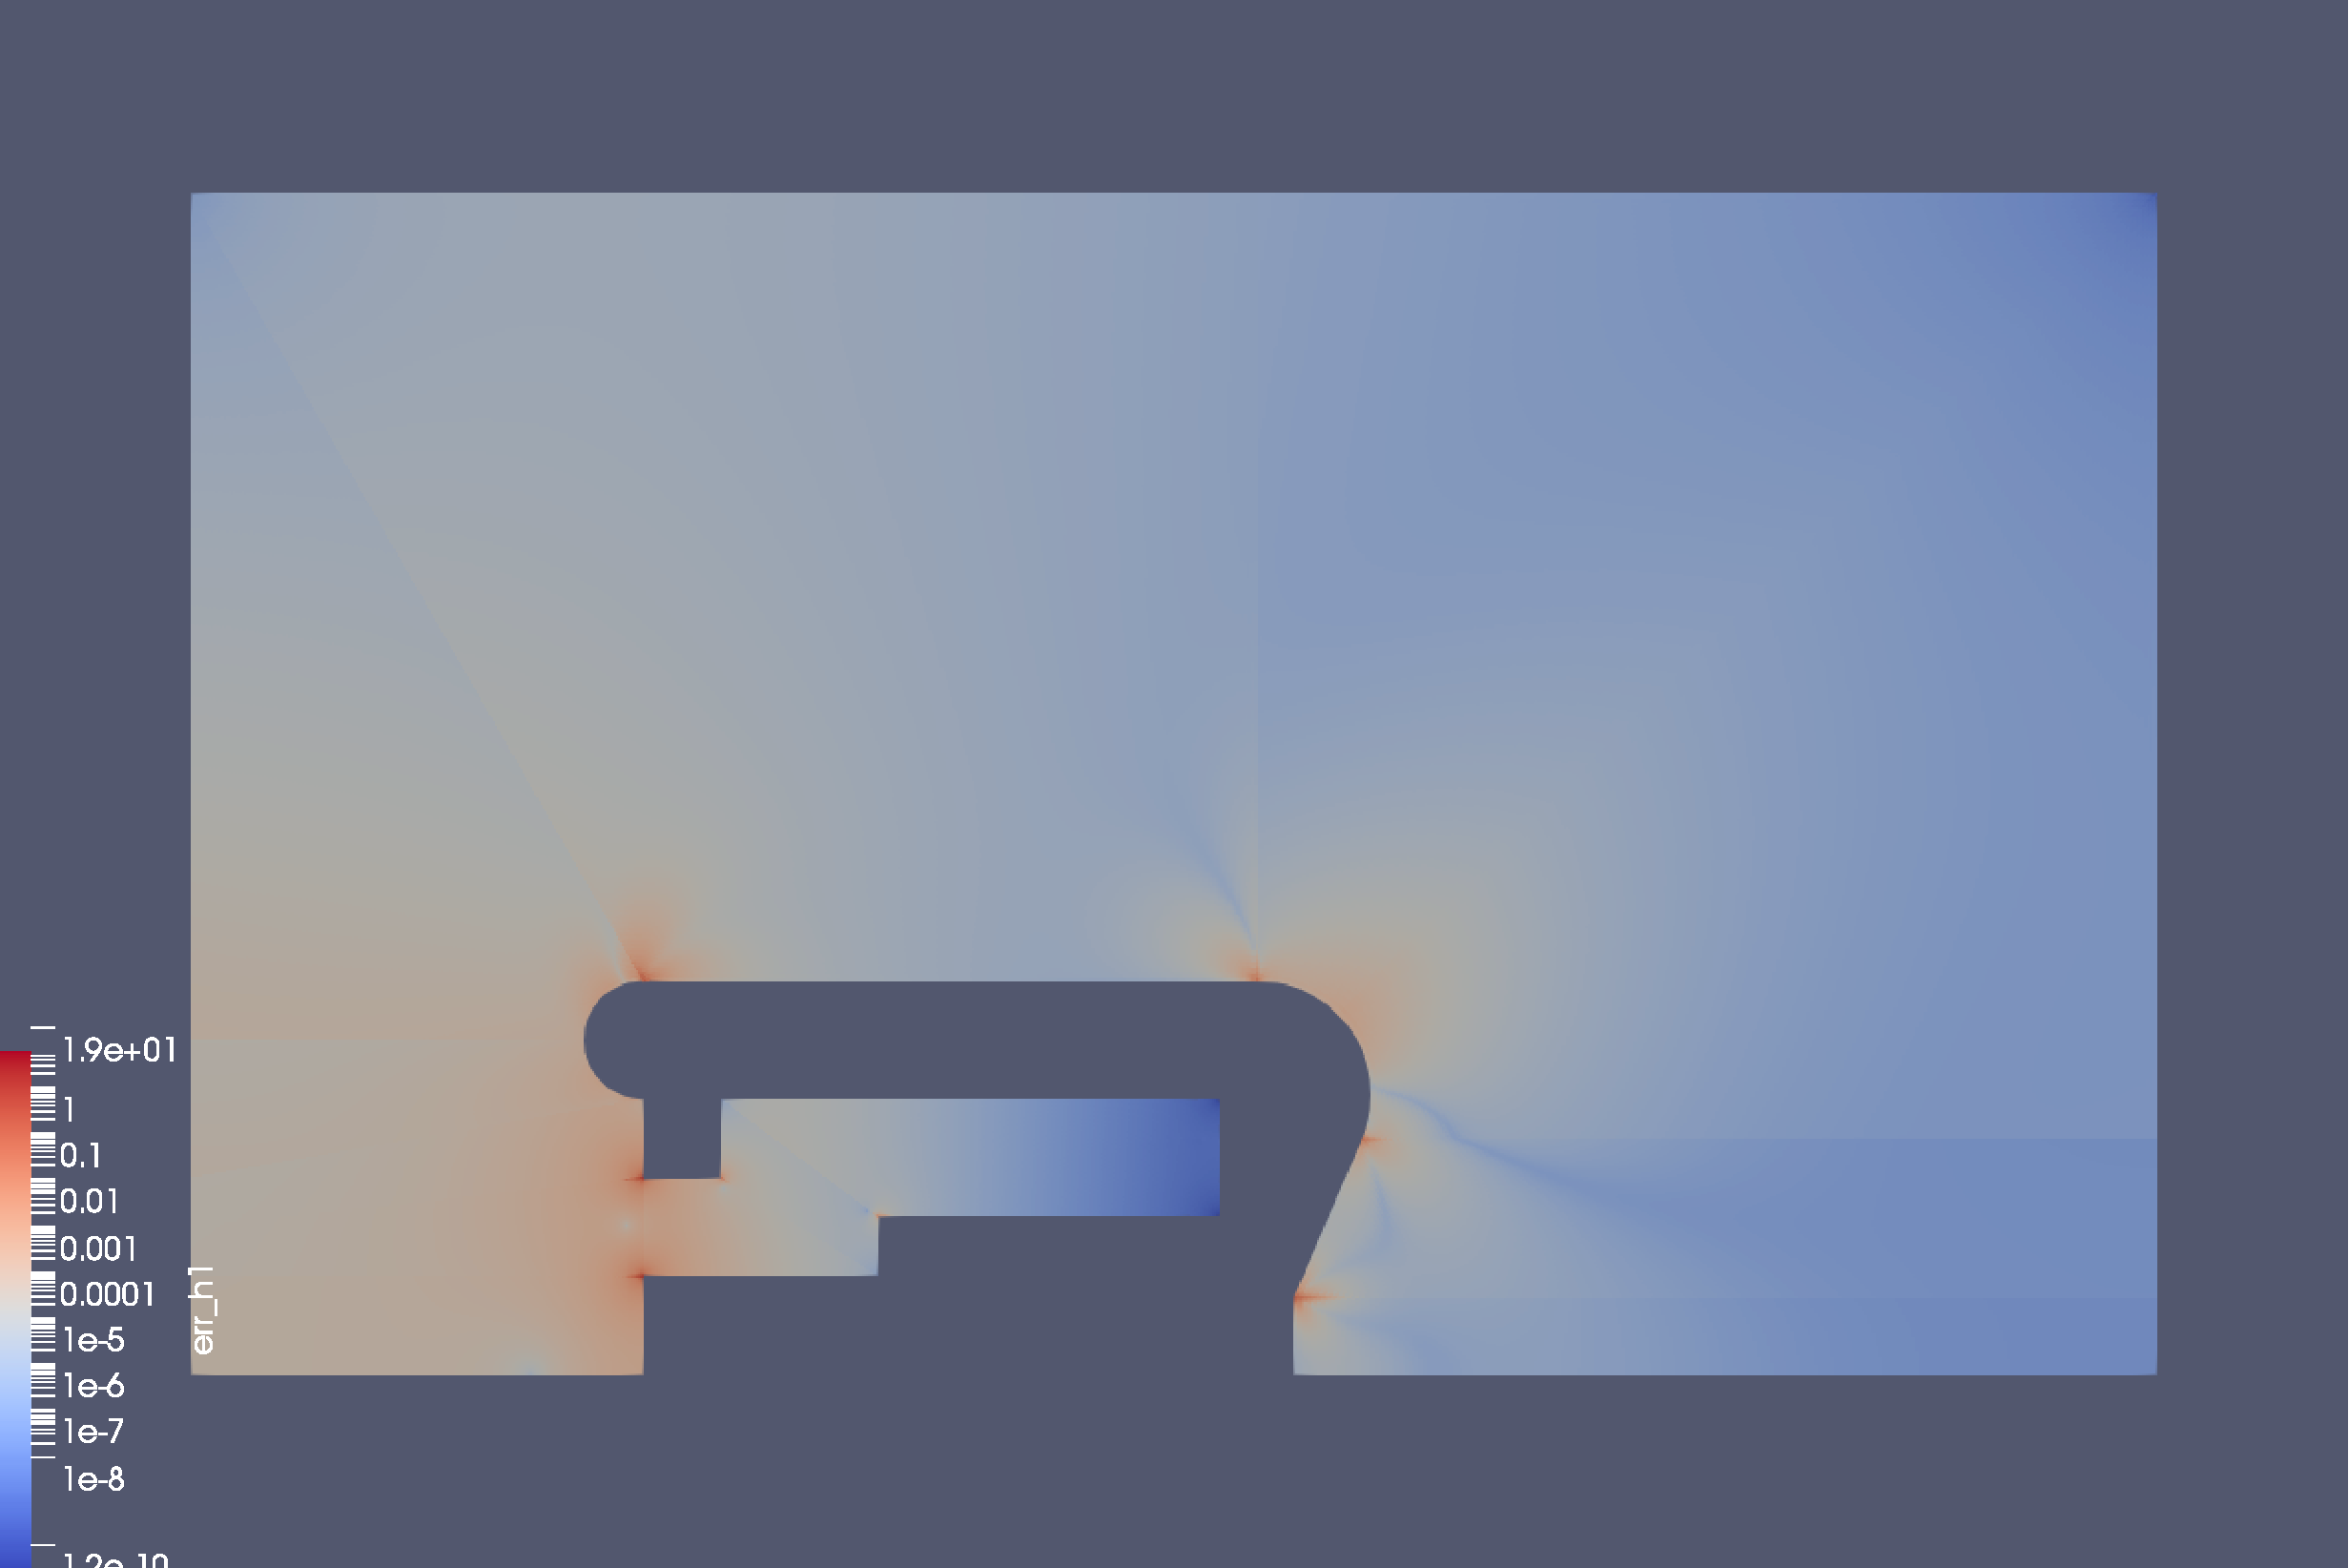
\includegraphics[width=\textwidth]{figures/insulator/error_elem}
  \caption{Absolute error of the electric field on every element.}
  \label{fig:error_elem}
\end{figure}
\end{center}
